\documentclass[12pt, parskip=half-]{scrartcl}
% \usepackage{showframe}
\usepackage[margin=1cm]{geometry}
\usepackage[french]{babel}
\usepackage[T1]{fontenc}
\usepackage[utf8]{inputenc}
\usepackage{mathtools}
\usepackage{tabularray}
\usepackage{enumitem}
\usepackage{graphicx}
\usepackage[charter]{mathdesign}
\usepackage{tikz}
\pagestyle{empty}

\begin{document}
\foreach \i in {1,...,3}{
Le but consiste à retrouver les cases noires dans chaque grille. Les chiffres donnés sur le côté et en haut de la grille vous donnent des indices. Ils indiquent la taille des blocs de cases noires de la ligne ou de la colonne sur laquelle ils se trouvent.

Par exemple 3,4 à gauche d'une ligne indique qu'il y a, de gauche à droite, un bloc de 3 cases noires puis un bloc de 4 cases noires sur cette ligne.

En revanche, ce qui n'est pas mentionné et qui fait la difficulté, est le nombre de cases blanches entre les cases noires. On sait simplement qu'il y en a au moins une.

Exemple : 

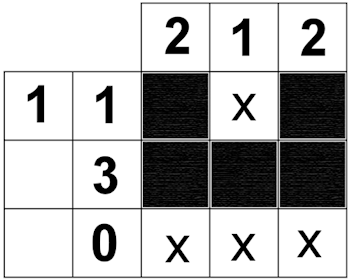
\includegraphics{img/exemple.png}

\dotfill

}
\newpage

\fbox{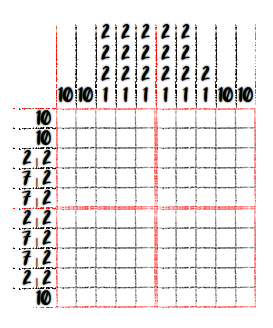
\includegraphics[height=8cm, width=8cm]{img/3.png}}
\fbox{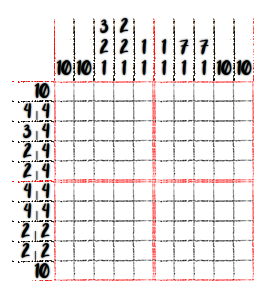
\includegraphics[height=8cm, width=8cm]{img/1.png}}

\fbox{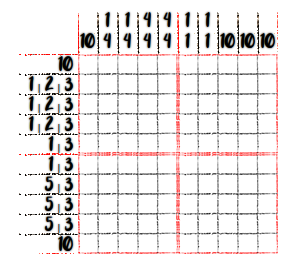
\includegraphics[height=8cm, width=8cm]{img/4.png}}
\fbox{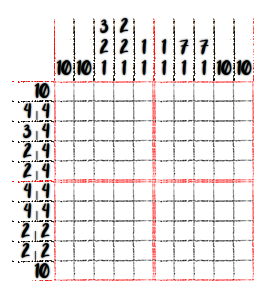
\includegraphics[height=8cm, width=8cm]{img/1.png}}

\fbox{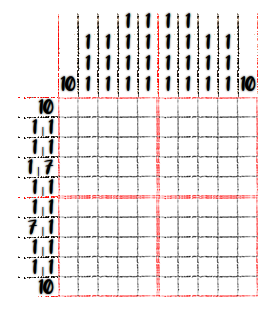
\includegraphics[height=8cm, width=8cm]{img/5.png}}

\end{document}